\documentclass{article}

\usepackage[utf8]{inputenc}
\usepackage[T1]{fontenc}
\usepackage{amsmath}
\usepackage{amsthm}
\usepackage{amssymb}
\usepackage{mathtools}
\usepackage{tikz}
\usepackage{setspace}
\usepackage{listings}
\usepackage{makeidx}
\usepackage{float}

\newcommand{\supp}{\mathrm{supp}}
\newcommand{\Z}{\mathbb{Z}}
\newcommand{\im}{\mathrm{Im}}

\usetikzlibrary{arrows,chains,matrix,positioning,scopes}
\makeatletter
\tikzset{join/.code=\tikzset{after node path={%
\ifx\tikzchainprevious\pgfutil@empty\else(\tikzchainprevious)%
edge[every join]#1(\tikzchaincurrent)\fi}}}
\makeatother

\tikzset{>=stealth',every on chain/.append style={join},
         every join/.style={->}}
\tikzstyle{labeled}=[execute at begin node=$\scriptstyle,
   execute at end node=$]

\newtheorem{defi}{Definition}[section]
\newtheorem{lem}{Lemma}[section]
\newtheorem{conj}{Conjecture}[section]
\newtheorem{rem}{Remark}[section]
\newtheorem{prop}{Proposition}[section]
\newtheorem{thm}{Theorem}[section]
\newtheorem{cor}{Corollary}[section]
\newtheorem{expl}{Example}[section]

\usepackage{mathpazo}

\title{The disjoint cycle expansion of a simplex}
\author{Kai Renken \and Dmitry Kozlov}

\date{\today}

\begin{document}

\maketitle


\begin{abstract}
In \cite{3} Meshulam and Wallach proved the estimate
\[
\frac{n}{k+2}\leq h_k(\Delta^{[n]})\leq\left\lceil\frac{n}{k+2}\right\rceil
\]
where $h_k(\Delta^{[n]})$ denotes the $k$-th Cheeger constant of the simplex on $n$-vertices. They also showed that the lower bound is archieved if $n$ is divisible by $k+2$. In \cite{2} Kozlov showed, that for the first Cheeger constant of a simplex this lower bound is archieved in all cases when $n$ is not a power of $2$ and he gave an estimate for the case when $n$ is a power of $2$.\\
In this paper we introduce the disjoint cycle expansion, another generalization of the classical Cheeger constant of a graph, which is easier to handle than that original generalization. We show that all exact values and estimates which are known for the Cheeger constant of the simplex equal those for the disjoint cycle expansion. 
\end{abstract}

\section{Introduction}

Let us quickly recall the notion of the $k$-th Cheeger constant of a simplicial complex. Through this paper we always consider chain- and cochain groups with $\mathbb{Z}_2$-coefficients.\\

\begin{defi}
Let $X$ be a simplicial complex and $k\geq 1$. We denote the \textbf{norm} of a $k$-cochain $\varphi\in C^k(X)$ by $\|\varphi\|\coloneqq |\supp(\varphi)|$ and we call
\[
\|\varphi\|_{csy}\coloneqq\min\limits_{\psi\in C^{k-1}(X)}\|\delta^{k-1}(\psi)+\varphi\|
\]
the \textbf{cosystolic norm} of $\varphi$. Then we can define the $k$-th Cheeger constant of $X$ by:
\[
h_k(X)\coloneqq\min_{\substack{\varphi\in C^k(X)\\\varphi\notin\im(\delta^{k-1})}}\frac{\|\delta^k(\varphi)\|}{\|\varphi\|_{csy}}
\]
\end{defi}

Now, we can define the $k$-th disjoint cycle expansion of a simplicial complex.

\begin{defi}
Let $X$ be a simplicial complex, $k\geq 1$, and $\mathcal{F}\subset C_k(X)$ a family of cycles, whose supports are pairwise disjoint. For such a family of cycles let
\begin{footnotesize}
\[
P(\mathcal{F})\coloneqq\{\varphi\in C^k(X):|\supp(\varphi)\cap\supp(F)|=1\text{ for all }F\in\mathcal{F}\text{ and }\supp(\varphi)\subset\bigcup\limits_{F\in\mathcal{F}}\supp(F)\}
\]
\end{footnotesize}
denote the set of all cochains constructed by all possible choices of one simplex per cycle in the family $\mathcal{F}$. Then we define
\[
\gamma_{\mathcal{F}}\coloneqq\frac{\min\limits_{\varphi\in P(\mathcal{F})}\|\delta^k(\varphi)\|}{|\mathcal{F}|}
\]
and we call
\[
\gamma_k(X)\coloneqq\min\limits_{\mathcal{F}\in\mathfrak{C}}\gamma_{\mathcal{F}}
\]
the $k$-th \textbf{disjoint cycle expansion} of $X$, where $\mathfrak{C}$ is the collection of all families of cycles in $C_k(X)$ with pairwise disjoint supports.
\end{defi}

To explain the relation between the $k$-th Cheeger constant and the $k$-th disjoint cycle expansion of a simplicial complex, we have to recall the notion of hitting sets and hitting numbers of families of sets and families of cycles and the cycle detection theorem (see \ref{proposition1}) which was stated by Kozlov in \cite{1}.

\begin{defi}
Let $V$ be some set and $\mathcal{F}\subseteq 2^V$ a family of subsets of $V$. A subset $P\subseteq V$ is called a \textbf{hitting set} of $\mathcal{F}$ if we have $P\cap F\neq\emptyset$ for all $F\in\mathcal{F}$. The minimal cardinality which a hitting set of $\mathcal{F}$ can attain is called the \textbf{hitting number} of $\mathcal{F}$, denoted by $\tau(\mathcal{F})$.
\end{defi}

\begin{defi}
Let \(X\) be a simplicial complex and \(\mathcal{F}\subseteq C_k(X)\) a family of \(k\)-chains. The \textbf{hitting sets} and the \textbf{hitting number} of \(\mathcal{F}\) are defined as the hitting sets and the hitting number of the family \(\left\{\supp(F):F\in\mathcal{F}\right\}\).
\end{defi}

\begin{prop}[The cycle detection theorem]\label{proposition1}
Let $X$ be a simplicial complex, $k\geq 1$, and $\varphi\in C^k(X)$. Let now $\mathcal{F}=\left\{\alpha_1,\ldots,\alpha_t\right\}$ be a family of $k$-cycles in $C_k(X)$, such that $\left\langle\varphi,\alpha_i\right\rangle=1$ for all $1\leq i\leq t$, then we have:
\[
\|\varphi\|_{csy}\geq\tau(\mathcal{F})
\]
\begin{proof}
Let $\psi\in C^{k-1}(X)$, then for any $1\leq i\leq t$ we have:
\begin{align}
\langle\varphi+\delta^{k-1}(\psi),\alpha_i\rangle&=\langle\varphi,\alpha_i\rangle+\langle\delta^{k-1}(\psi),\alpha_i\rangle\notag\\
&=\langle\varphi,\alpha_i\rangle+\langle\psi,\partial_{k-1}(\alpha_i)\rangle\notag\\
&=\langle\varphi,\alpha_i\rangle+\langle\psi,0\rangle\notag\\
&=\langle\varphi,\alpha_i\rangle=1\notag
\end{align}
This means that we have $\supp(\varphi+\delta^{k-1}(\psi))\cap \supp(\alpha_i)\neq\emptyset$ for all $1\leq i\leq t$, so $\supp(\varphi+\delta^{k-1}(\psi))$ is a hitting set of $\mathcal{F}$ and we get:
\[
\|\varphi+\delta^{k-1}(\psi)\|=|\supp(\varphi+\delta^{k-1}(\psi))|\geq\tau(\mathcal{F})
\]
Since $\psi$ was chosen arbitrarily we are done.
\end{proof}
\end{prop}

The cycle detection theorem can now be used to describe a fundamental relation between the Cheeger constant and the disjoint cycle expansion.

\begin{prop}\label{proposition2}
Let $X$ be a simplicial complex and $k\geq 1$, then we have:
\[
h_k(X)\leq\gamma_k(X)
\]
\begin{proof}
Let $\mathcal{F}\subset C_k(X)$ be a family of cycles with pairwise disjoint supports and $\varphi\in P(\mathcal{F})$. Then we have $\tau(\mathcal{F})=|\mathcal{F}|$ and by the cycle detection theorem we get $\|\varphi\|_{csy}=|\mathcal{F}|$. Hence, we have $h_k(X)\leq\gamma_k(X)$.
\end{proof}
\end{prop}

\section{The main results}

\begin{thm}\label{theorem1}
Let $n\geq 3$ and $1\leq k\leq n-2$, then we have:
\[
\frac{n}{k+2}\leq\gamma_k(\Delta^{[n]})\leq\left\lceil\frac{n}{k+2}\right\rceil
\]
\begin{proof}
To prove the lower bound, we only have to combine Proposition \ref{proposition2} with the fact that $h_k(\Delta^{[n]})\geq\frac{n}{k+2}$ holds (see \cite{2}). To prove the lower bound, we only have to combine Proposition \ref{proposition2} with the fact that $h_k(\Delta^{[n]})\geq\frac{n}{k+2}$ holds (see \cite{2}). To prove the upper bound let $n$ be divisible by $k+2$. By Theorem \ref{theorem2} we know that we have $\gamma_k(\Delta^{[n]})=\frac{n}{k+2}$. Consider the set of cycles $\mathcal{F}$ and $\varphi\in P(\mathcal{F})$ as constructed in the proof of Theorem \ref{theorem2}. Now, remove an arbitrary non-isolated vertex (i.e. a vertex which participates in $\supp(\varphi)$, all simplices from $\supp(\varphi)$ which contain this vertex and all cycles from $\mathcal{F}$ which contain this vertex. We get a new family of cycles $\mathcal{F}'$ and a new $\varphi'\in P(\mathcal{F}')$ such that we have
\[
\frac{\|\delta^k(\varphi')\|}{|\mathcal{F}'|}=\frac{n}{k+2}=\left\lceil\frac{n-1}{k+2}\right\rceil.
\]
We can proceed removing vertices this way getting the same results.
\end{proof}
\end{thm}

\begin{thm}\label{theorem2}
Let $k+2$ devide $n$, then we have:
\[
\gamma_k(\Delta^{[n]})=\frac{n}{k+2}
\]
\begin{proof}
See \cite{1}.
\end{proof}
\end{thm}

\begin{thm}\label{theorem3}
Let $n$ not be a power of $2$, then we have:
\[
\gamma_1(\Delta^{[n]})=\frac{n}{3}
\] 
\begin{proof}
Since $n$ is not a power of $2$ we can write it as $n=c(2t+1)$. Now consider the staircase graph $G_n(\lambda)$ given by the partition $\lambda=c\cdot\text{cor}(t)$. For the definition of staircase graphs and partitions, see \cite{2}. Since $G_n(\lambda)$ is bipartite we can partition the vertices of $G_n(\lambda)$ as $[n]=A\cup B\cup C$, with $A=\{v_1,\ldots,v_{ct}\}$, $B=\{w_1,\ldots,w_{ct}\}$ and $C=\{x_1,\ldots,x_c\}$, such that $C$ is the set of all isolated vertices, and all edges of $G_n(\lambda)$ are contained in $E_{G_n(\lambda)}(A,B)$. Construct a family of cycles in $C_1(\Delta^{[n]})$ with pairwise disjoint supports as follows:\\
For all edges $(v_i,w_j)$ satisfying $i+j\leq ct$, such that $(v_{ct-j+1},w_{ct-i+1})$ is not an edge in $G_n(\lambda)$ consider the cycle
\[
C_{ij}\coloneqq (v_i,w_j)+(v_{ct-j+1},w_{ct-i+1})+(v_i,v_{ct-j+1})+(w_j,w_{ct-i+1})
\]
For all edges $e_{ij}=(v_i,w_j)$ satisfying $i+j\leq ct+1$, such that $e'_{ij}=(v_{ct-j+1},w_{ct-i+1})$ is also an edge in $G_n(\lambda)$ (for $i+j=ct+1$ they are equal), the set
\[
D\coloneqq\{e_{ij}, e'_{ij}:i+j\leq ct+1\text{, }e_{ij}\text{ and }e'_{ij}\text{ are edges in }G_n(\lambda)\}
\] can be partitioned into $t$ sets $B_1,\ldots,B_t$, each containing $c^2$ edges:
\[
B_k\coloneqq\{(v_i,w_j):(k-1)c+1\leq i\leq kc\text{, }c(t-k)+1\leq j\leq c(t-k+1)\}
\]
Now, each vertex from $A\cup B$ is only contained in edges from exactly one of the sets $B_k$. This means that for any $l=1,\ldots,c$ and any pair of edges $(v_i,w_j)\in B_{k_1}$ and $(v_{i'},w_{j'})\in B_{k_2}$ ($k_1\neq k_2$) the supports of the cycles $(v_i,w_j)+(v_i,x_l)+(w_j,x_l)$ and $(v_{i'},w_{j'})+(v_{i'},x_l)+(w_{j'},x_l)$ are disjoint. Furthermore, each set $B_k$ itself is a complete balanced bipartite graph (i.e. a graph in which each of the $c$ vertices from $A$ is adjacent to each of the $c$ vertices from $B$) so we can partition it into $c$ sets $B_k^1,\ldots,B_k^c$, such that all edges in $B_k^l$ are disjoint, for every $l=1,\ldots,c$. Thus, the supports of the cycles $(v_i,w_j)+(v_i,x_l)+(w_j,x_l)$ are pairwise disjoint for all $(v_i,w_j)\in B_k^l$. The family of all these cycles united with the cycles $C_{ij}$ we defined before gives a family of cycles with pairwise disjoint supports, such that every edge of $G_n(\lambda)$ is contained in exactly one cycle and every cycle containes exactly one of the edges from $G_n(\lambda)$. Since the number of cycles in this family equals the number of edges in $G_n(\lambda)$ and we know that we have $h(G_n(\lambda))=\frac{n}{3}$ by \cite{2} (Theorem 4.2.) we get $\gamma_1(\Delta^{[n]})\leq\frac{n}{3}$ and by Proposition \ref{proposition2} we have $\gamma_1(\Delta^{[n]})=\frac{n}{3}$.
\end{proof}
\end{thm}

\begin{expl}
Let $n=10$ and consider the staircase graph $G_{10}(\lambda)$ with $\lambda=2\cdot\text{cor}(2)$ as shown in Figure \ref{figure1:Figure 1} ($v_i$ and $w_j$ are adjacent if and only if there is a box in column $i$ and row $j$ and the $x_i$'s are isolated vertices). Then, intuitively speaking, for every edge represented by a box for which there is no box on the other side of the diagonal
\[
(v_1,w_4),(v_2,w_3),(v_3,w_2),(v_4,w_1)
\]
we can "use" the missing boxes to construct cycles for these edges as we did in the first part of the proof of Theorem \ref{theorem3}. This means, we get the family of cycles:
\begin{align}
\{&(v_1,w_1)+(v_4,w_4)+(v_1,v_4)+(w_1,w_4),(v_2,w_2)+(v_3,w_3)+(v_2,v_3)+(w_2,w_3),\notag\\
&(v_1,w_2)+(v_3,w_4)+(v_1,v_3)+(w_2,w_4),(v_2,w_1)+(v_4,w_3)+(v_2,v_4)+(w_1,w_3)\}\notag
\end{align}
For the remaining edges, according to the second part of the proof we use the isolated vertices to construct cycles and we get the family of cycles:
\begin{align}
\{&(v_1,w_4)+(v_1,x_1)+(w_4,x_1),(v_2,w_3)+(v_2,x_1)+(w_3,x_1),\notag\\
&(v_3,w_2)+(v_3,x_1)+(w_2,x_1),(v_4,w_1)+(v_4,x_1)+(w_1,x_1),\notag\\
&(v_1,w_3)+(v_1,x_2)+(w_3,x_2),(v_2,w_4)+(v_2,x_2)+(w_4,x_2),\notag\\
&(v_3,w_1)+(v_3,x_2)+(w_1,x_2),(v_4,w_2)+(v_4,x_2)+(w_2,x_2)\}\notag
\end{align}
Uniting both families gives a family of cycles $\mathcal{F}$, whose supports are pairwise disjoint and such that every edge of $G_{10}(\lambda)$ is contained in the support of exactly one cycle. If we consider $\varphi\in C^1(\Delta^{[10]})$ as the characteristic cochain of the chain respresented by $G_{10}(\lambda)$, then we have $\|\delta^1(\varphi)\|=40$ and we have $|\mathcal{F}|=12$, so we get:
\[
\gamma_{\mathcal{F}}=\frac{40}{12}=\frac{10}{3}
\]

\begin{figure}[ht]
\centering
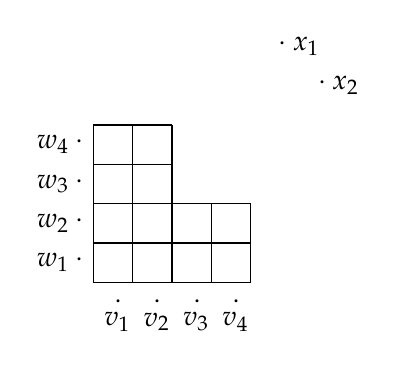
\begin{tikzpicture}[scale=0.5, line width=0.5pt]
  \draw (0,0) grid (4,1);
  \draw (0,0) grid (4,2);
  \draw (0,0) grid (2,3);
  \draw (0,0) grid (2,4);
  
  \node[left] (A) at (1.2,-1) {$v_1$};
  \node[left] (B) at (2.2,-1) {$v_2$};
  \node[left] (C) at (3.2,-1) {$v_3$};
  \node[left] (D) at (4.2,-1) {$v_4$};
  
  \node[left] (A') at (1,-0.5) {$\cdot$};
  \node[left] (B') at (2,-0.5) {$\cdot$};
  \node[left] (C') at (3,-0.5) {$\cdot$};
  \node[left] (D') at (4,-0.5) {$\cdot$};
  
  \node[left] (F) at (0,0.5) {$w_1\:\cdot$};
  \node[left] (G) at (0,1.5) {$w_2\:\cdot$};
  \node[left] (H) at (0,2.5) {$w_3\:\cdot$};
  \node[left] (I) at (0,3.5) {$w_4\:\cdot$};
  
  \node[left] (J) at (6,6) {$\cdot\:x_1$};
  \node[left] (K) at (7,5) {$\cdot\:x_2$};
  
\end{tikzpicture}
  \caption{The staircase graph $G_{10}(\lambda)$ with $\lambda=2\cdot\text{cor}(2)$}
  \label{figure1:Figure 1}
\end{figure}
\end{expl}

\begin{thm}\label{theorem4}
Let $n$ be a power of $2$, then we have:
\[
\gamma_1(\Delta^{[n]})\leq\frac{n^3-4n}{3n^2-24}
\]
\begin{proof}
Let $n=2^k$. Then we can write $n-1=2t+1$ with $t$ being odd. Now construct a staircase graph as follows:
Consider the staircase graph $G_n(\lambda)$ with $\lambda=\text{cor}(t)$ and a partitioning of its vertices $[n]=A\cup B\cup C$ with $A=\{v_1,\ldots,v_t\}$, $B=\{w_1,\ldots,w_t\}$ and $C=\{x_1,x_2\}$ as described in the proof of Theorem \ref{theorem3}. Let $E'$ be the set of edges in $G_n(\lambda)$. Now define
\[
E\coloneqq\{(v_2,w_t),(v_4,w_{t-2}),(v_6,w_{t-4}),\ldots,(v_{t-1},w_3)\},
\]
then we can construct a family of pairwise edge-disjoint cycles the same way we did in the proof of Theorem \ref{theorem3} which satisfy the conditions of the cycle detection theorem and we get
\[
|E|=\frac{n^2}{8}-1
\]
and
\[
|T(G)|=\frac{n^3-4n}{24}
\]
so we have
\[
\gamma_1(\Delta^{[n]})\leq\frac{|T(G)|}{|E|}=\frac{n^3-4n}{3n^2-24}
\]
\end{proof}
\end{thm}

\begin{thebibliography}{9}

\bibitem{1} Dmitry N. Kozlov, Roy Meshulam; Quantitative aspects of acyclicity

\bibitem{2} Dmitry N. Kozlov; The first Cheeger constant of a simplex

\bibitem{3} R. Meshulam, N. Wallach; Homological connectivity of random k-dimensional complexes

\end{thebibliography}

\end{document}


